%--------------------------------------------------------------------------------------------------
% architecture.tex
%
% This document define the frontespiece of the presentation
%
% author: Andrea Meneghinello
% version: 0.1
%--------------------------------------------------------------------------------------------------
\section{Architecture}
\begin{frame}{Architecture}
	\begin{columns}
		\begin{column}{0.6\textwidth}
			Developers have to:
			\begin{itemize}
				\item{\footnotesize{abandon ``monolithic'' architectures}}
				\item{\footnotesize{revisit Service Oriented Architecture (SOA)}}
				\begin{itemize}
					\item{\scriptsize{micro-services}}
				\end{itemize}
			\end{itemize}
		\end{column}
		\begin{column}{0.4\textwidth}
			\begin{figure}
				\centering{}
				
\includegraphics[scale=0.2]{images/think.png}
			\end{figure}
			\begin{flushright}
				\tiny{source: \url{http://goo.gl/DwpRhl}}
			\end{flushright}
		\end{column}
	\end{columns}
\end{frame}

\subsection{Micro-services}
\begin{frame}{Micro-services}
	\begin{columns}
		\begin{column}{0.6\textwidth}
			SOA and Cloud
			\begin{itemize}
				\item{\footnotesize{have common points}}
				\item{\footnotesize{we have to review services size $\rightarrow{}$ elasticity performance}}
				\begin{itemize}
					\item{\scriptsize{services $\rightarrow{}$ micro-services}}
				\end{itemize}
			\end{itemize}
		\end{column}
		\begin{column}{0.4\textwidth}
			\begin{figure}
				\centering{}
				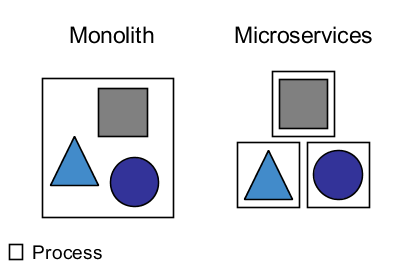
\includegraphics[scale=0.25]{images/micro-services.png}
			\end{figure}
			\begin{flushright}
				\tiny{source: \url{http://goo.gl/Z0i67L}}
			\end{flushright}
		\end{column}
	\end{columns}
\end{frame}

\subsection{Proposed architecture}
\begin{frame}{Proposed architecture}
	\begin{figure}
		\centering{}
		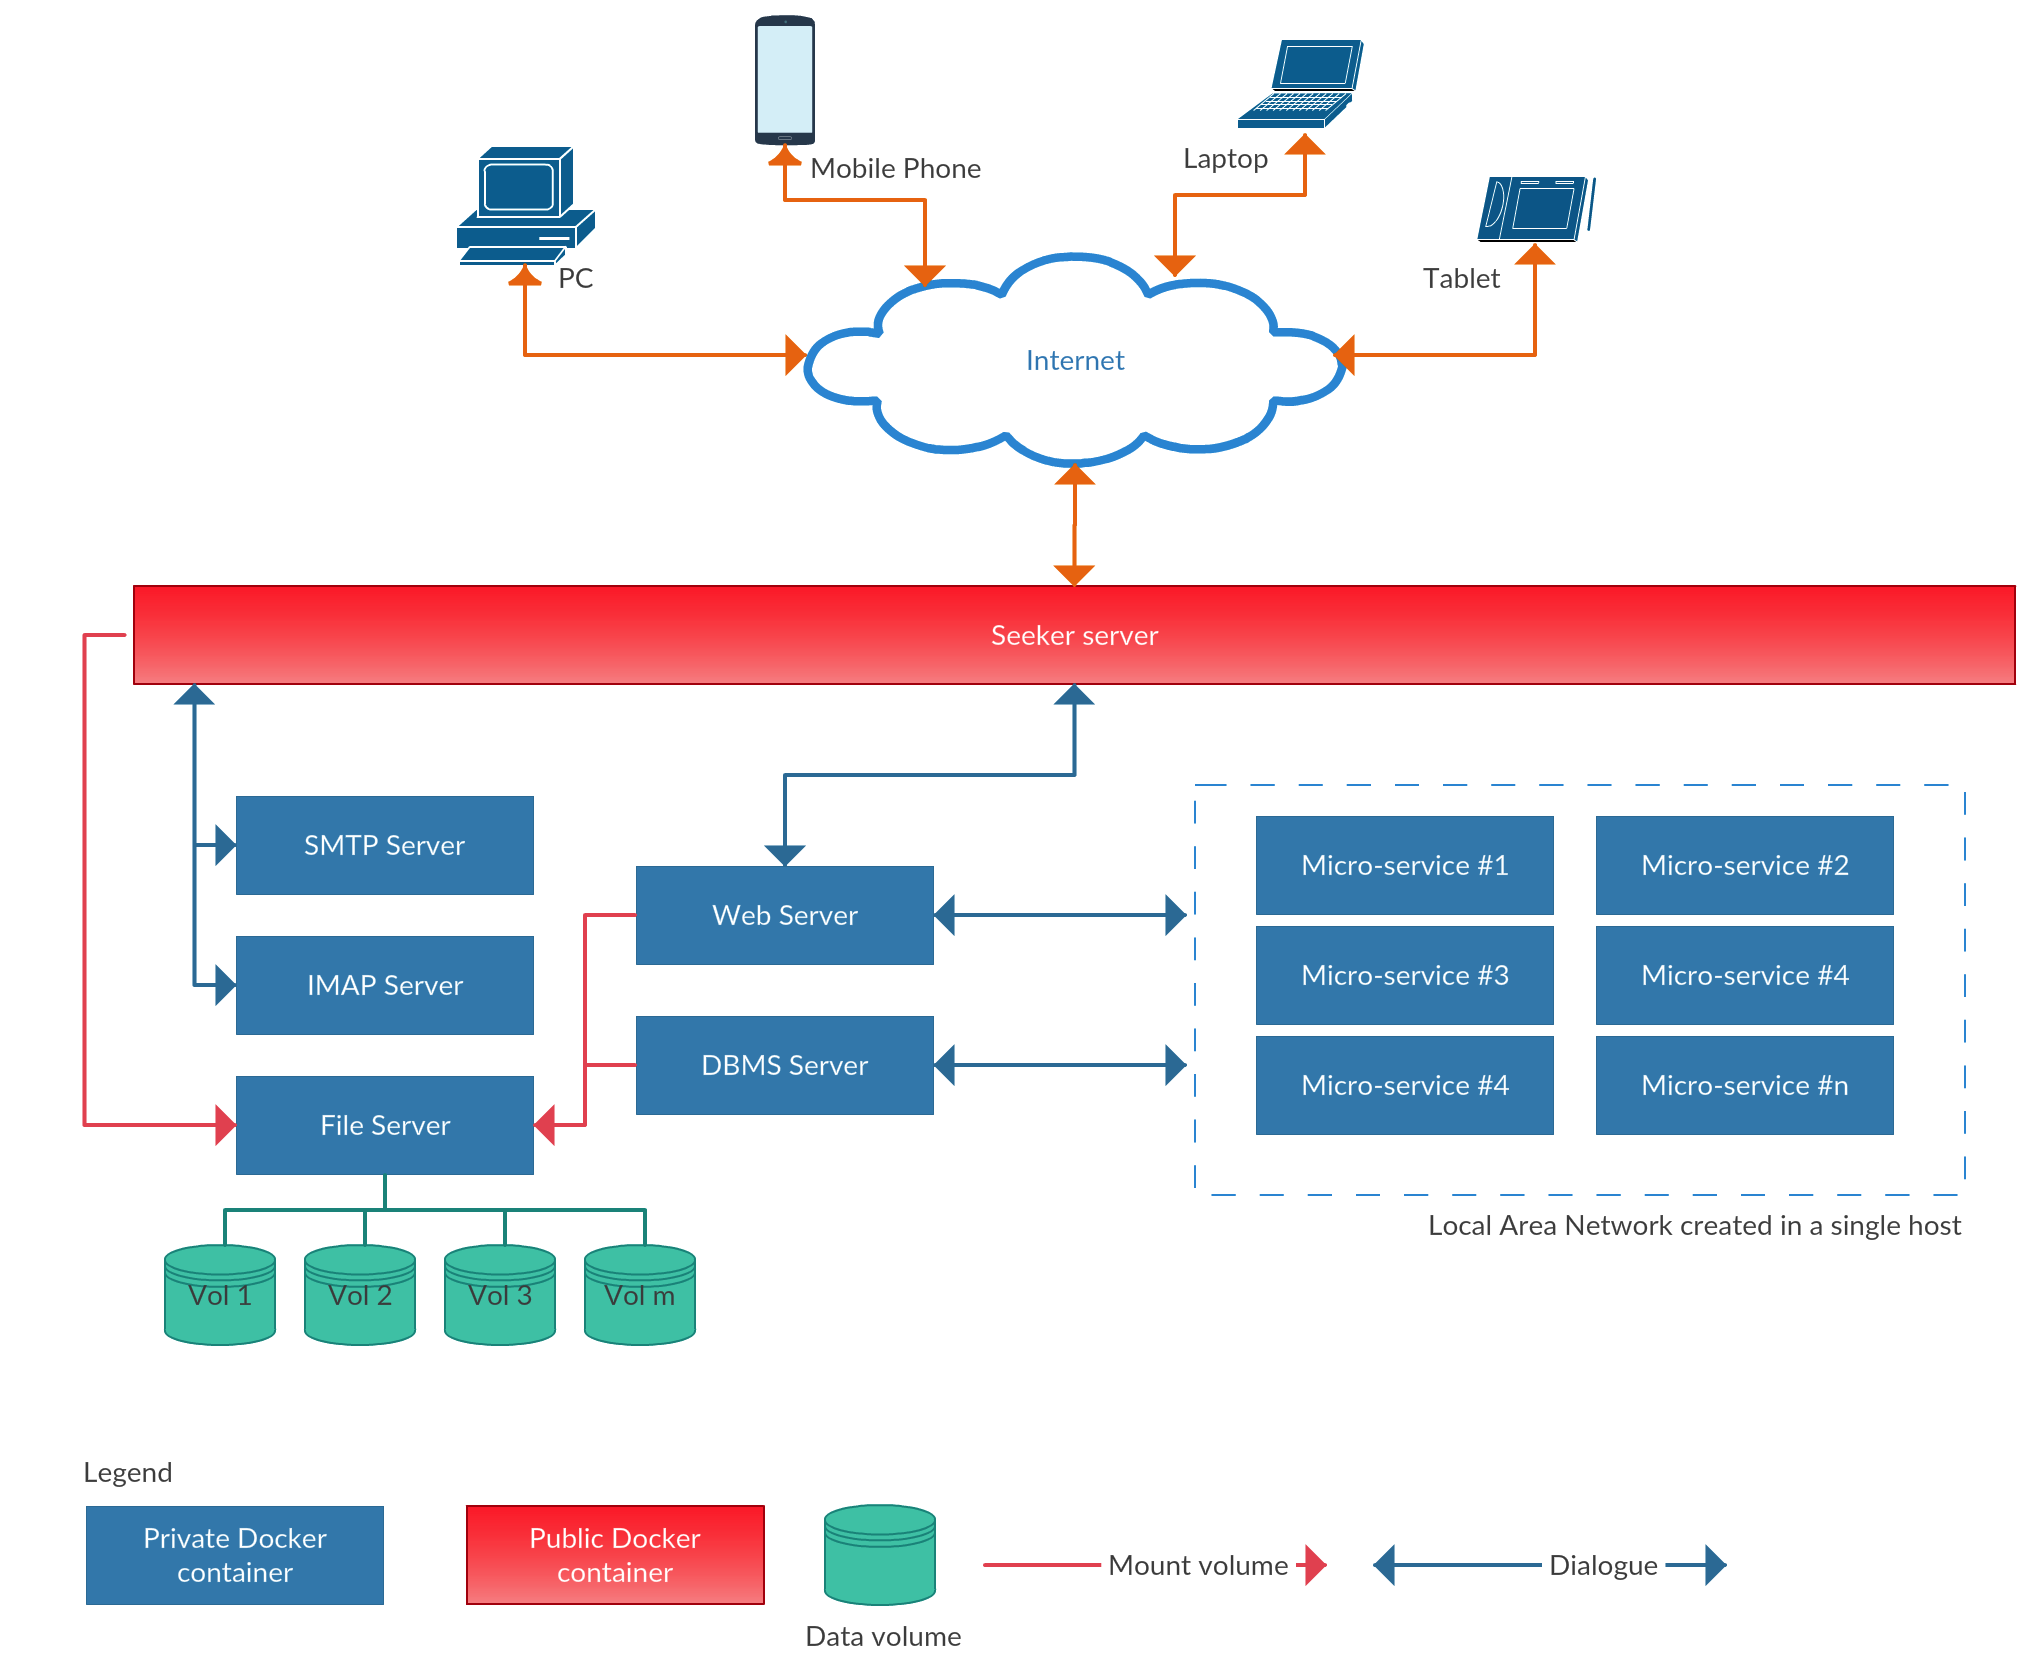
\includegraphics[scale=0.11]{images/architecture.png}
	\end{figure}
\end{frame}